\chapter{Results\label{ch:results}}

The signal yield is evaluated by fitting the data with a model that additively combines the signal
and background shapes, where the normalization for each component is a free parameter.
This is evaluated from a simultaneous fit to the $\Mgg$, $\Mggjjk$, and $\Mgg \times \Mjj$ spectra
for the low-mass resonant, high-mass resonant, and nonresonant searches, respectively.
From the signal-plus-background fit, the confidence level (CL)
for discovery or exclusion of double Higgs production is calculated.
To compute the upper limits on the production cross section, the modified frequentist approach
$\text{CL}_s$ is used with an asymptotic approximation, taking the profile likelihood as a test
statistic~\cite{CLS1,CLS2}. This calculation is discussed in Section~\ref{sec:resresults} for the
resonant search and in Section~\ref{sec:nonresresults} for the SM nonresonant search.

\section{Resonant Results\label{sec:resresults}}

\subsection{Low-mass Resonant Results}

In the low-mass resonant search,
no excess above the expectation is observed, so upper limits on the signal cross section are calculated.
The 95\% CL for observed and expected upper limits is shown in
Table~\ref{table:limits_lowmass} and Figure~\ref{fig:limits_lowmassres}
for both categories and for the high-purity category only.
The latter result is provided to simplify the comparison with new physics models where
the Higgs branching ratios for the $\Hgg$ and $\Hbb$ decays can be modified with respect to their
values in the SM.
The green and yellow bands represent the 1$\sigma$ and 2$\sigma$
confidence intervals around the expected limit. Theory expectations for Radion, RS1 KK-graviton, and 
bulk KK-graviton are shown, where the Radion expectation assumes $\text{BR}(R\rightarrow HH) =$~25\%
for all Radion masses above 300 GeV. Through comparison with the Graviton simulation,
the search is verified to be spin-independent, so theory expectations for both spin-0 and spin-2
hypotheses may be overlaid together.

\begin{table}[htbp!]
  \centering
  \renewcommand{\arraystretch}{1.4}
  \caption{Observed and median expected 95\% CL upper limits for $m_X \le 400$~GeV.}
  \begin{tabular}{ | c || c | c || c | c |}
\hline
$m_X$ (GeV) & Observed limit (fb) & Expected limit (fb) & Observed limit (fb) & Expected limit (fb) \\ \hline
 & & &  \multicolumn{2}{c|}{High-purity category only} \\ \hline
260 & 3.14 & 2.12 & 3.54 & 2.41 \\
270 & 2.70 & 2.40 & 3.07 & 2.74 \\
300 & 3.98 & 2.73 & 3.64 & 3.14 \\
350 & 1.67 & 2.23 & 2.17 & 2.66 \\
400 & 1.97 & 1.66 & 3.40 & 2.01 \\ \hline
\end{tabular}

  \label{table:limits_lowmass}
\end{table}

\begin{figure}[htbp!]
 \begin{center}
   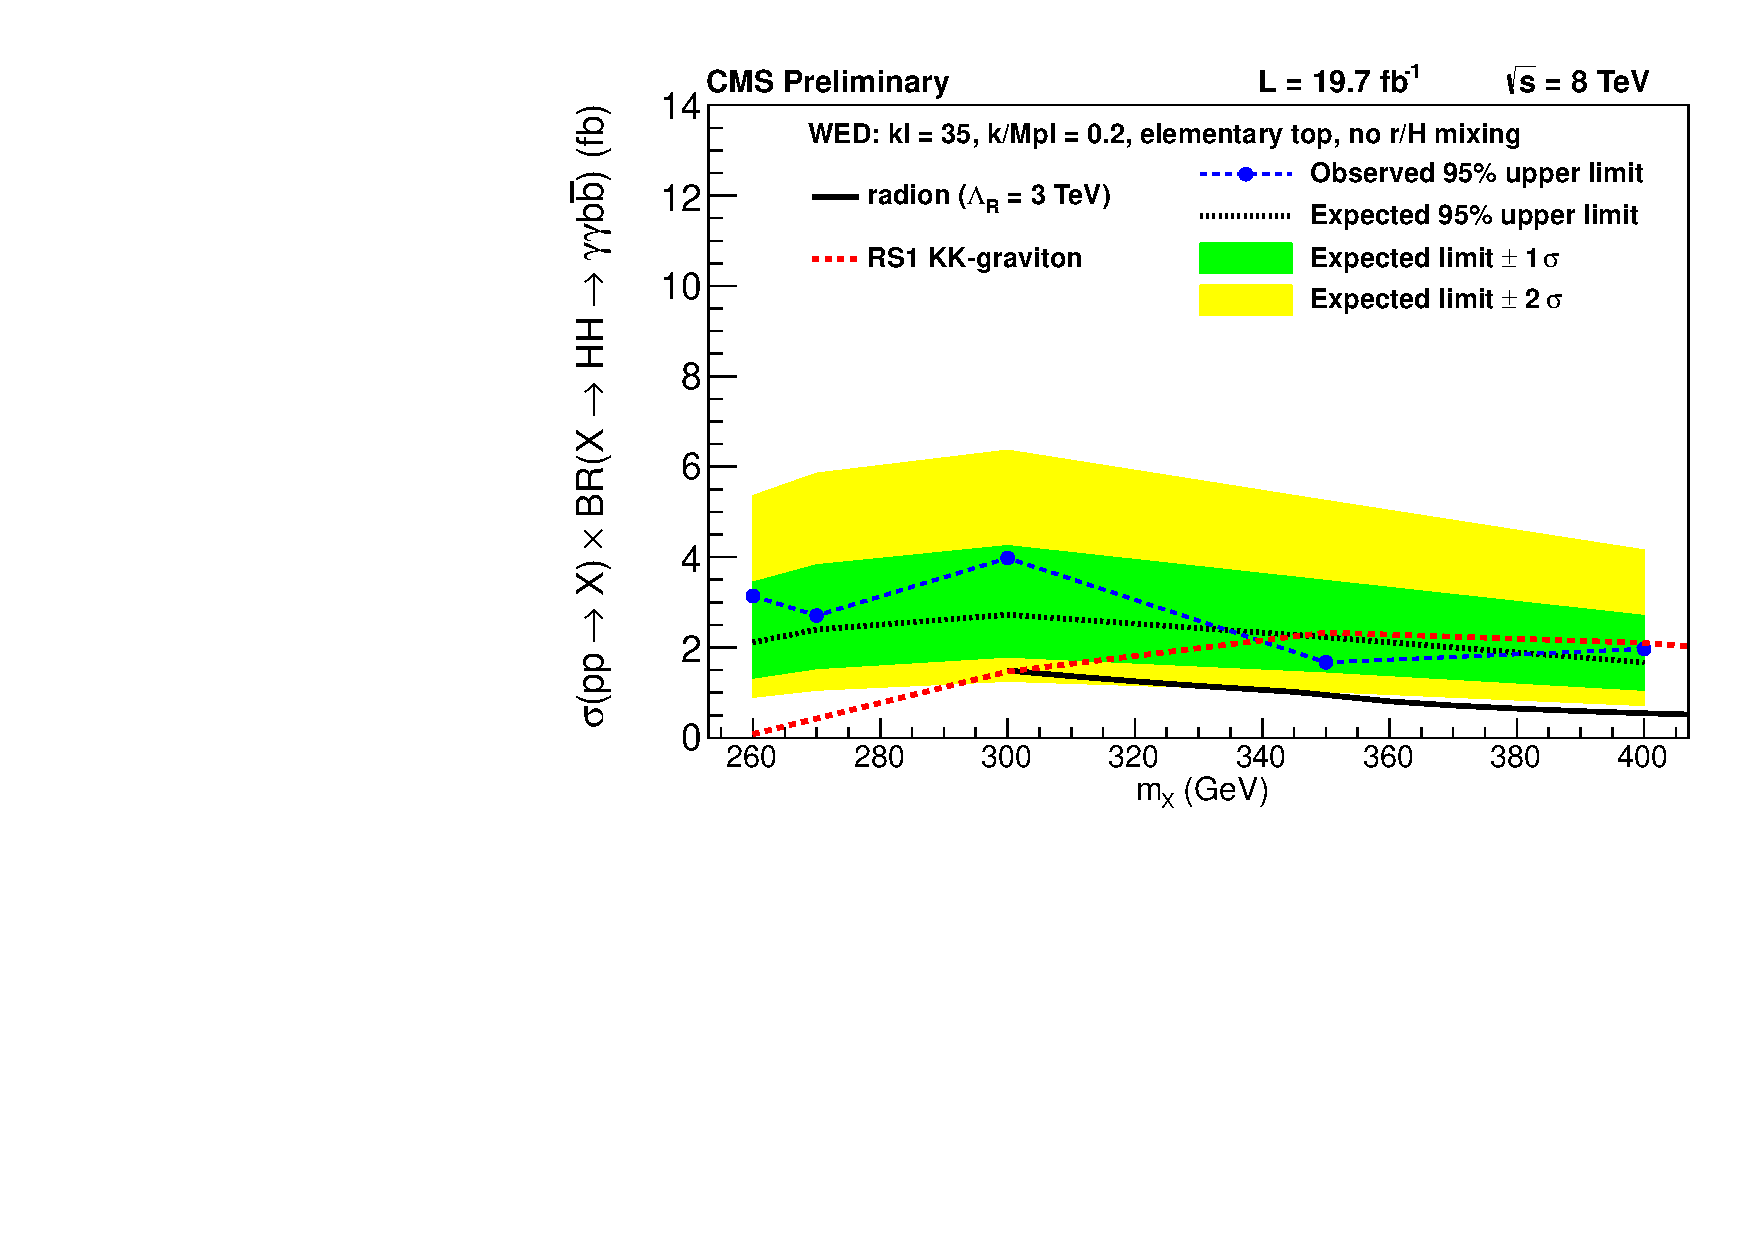
\includegraphics[width=0.8\textwidth]{figures/results/WP4_cutbased_low_all.pdf}
   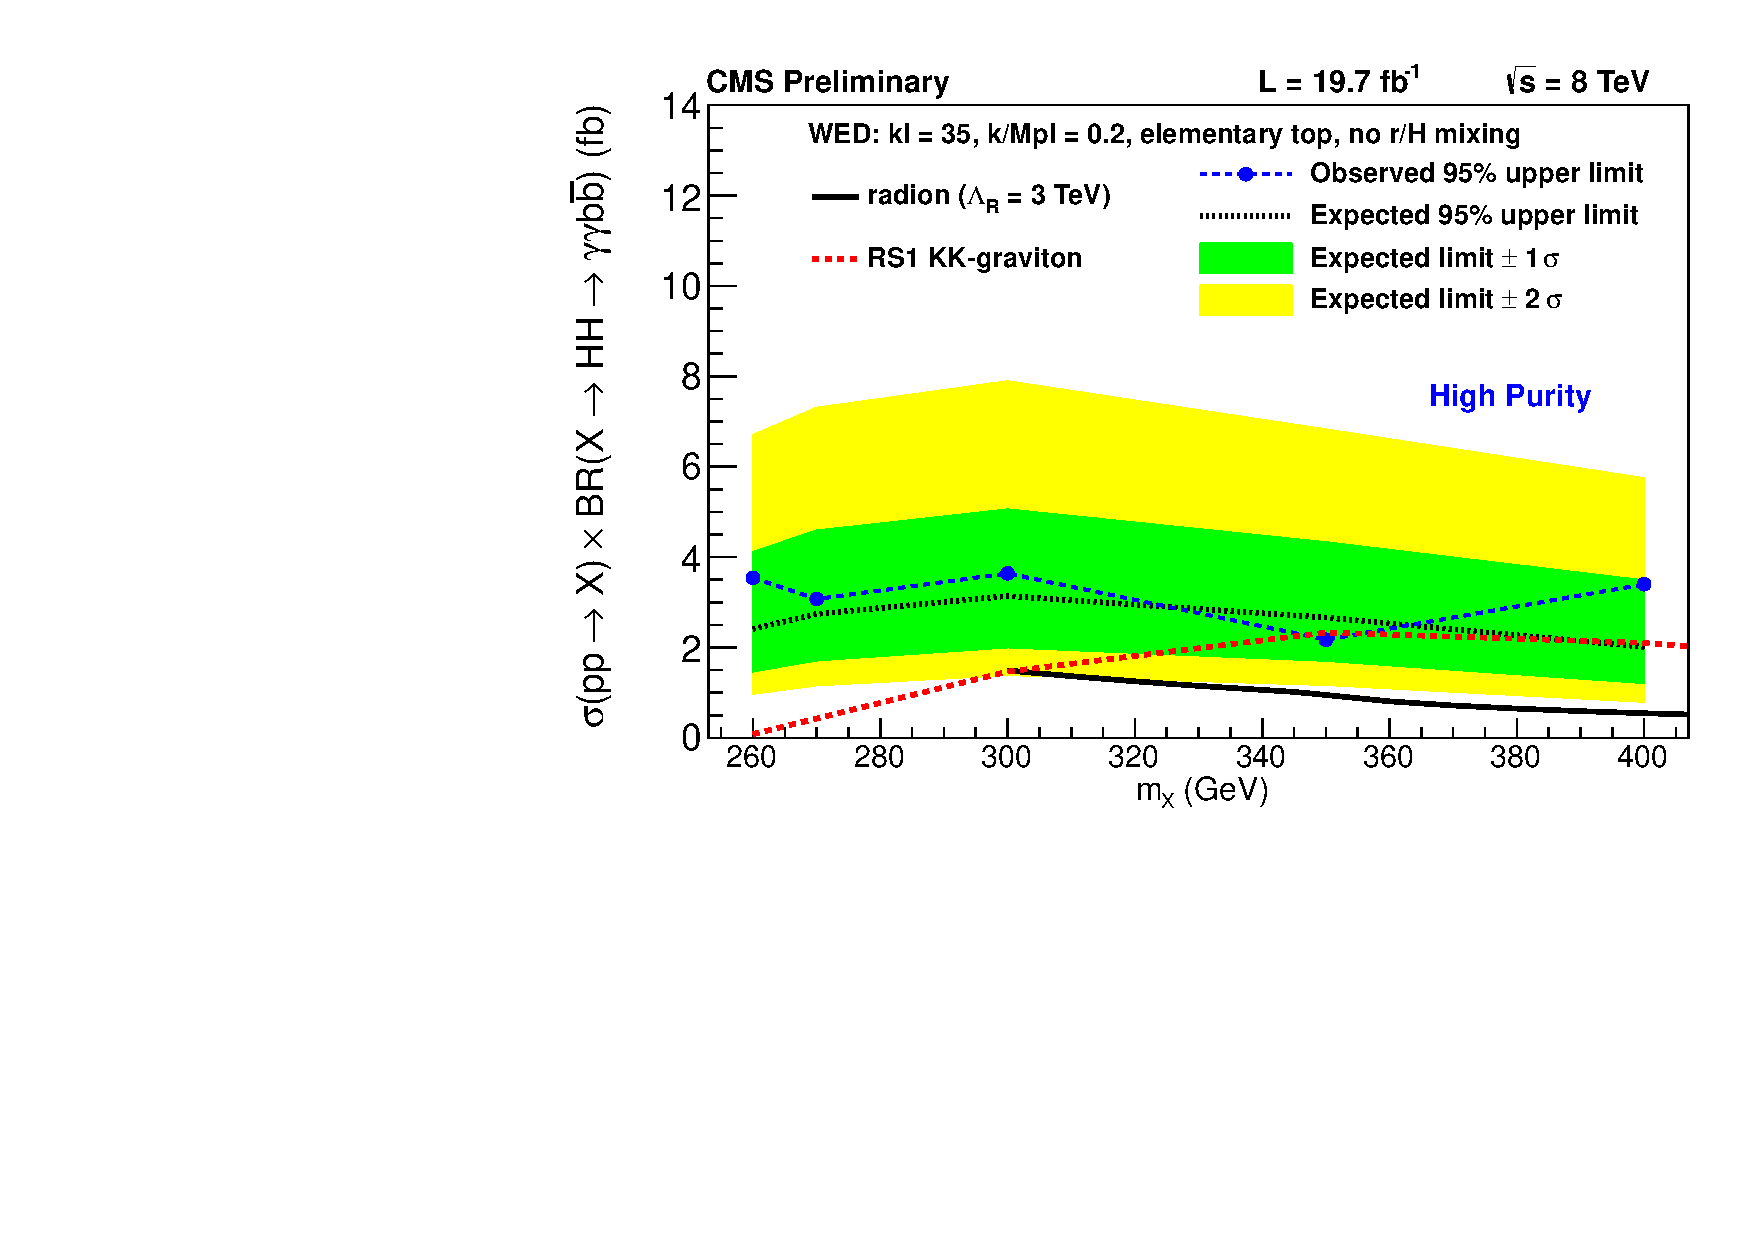
\includegraphics[width=0.8\textwidth]{figures/results/WP4_cutbased_low_base_onecat.pdf}
 \end{center}
\caption{Expected 95\% CL upper limits on the cross section times branching ratio
$\sigma(pp\rightarrow X) \times \text{BR}( X \rightarrow HH \rightarrow \gamma\gamma b\bar{b})$.
Theory lines corresponding to WED models with Radion, RS1 KK-graviton, and bulk KK-graviton are
overlaid. Limits from both categories (top) and high-purity category only (bottom) are shown.
The results are obtained using the asymptotic $\text{CL}_s$ approach.}
\label{fig:limits_lowmassres}
\end{figure}

\subsection{High-mass Resonant Results}

In the high-mass resonant search,
no excess above the expectation is observed, so upper limits on the signal cross section are calculated.
The 95\% CL for expected and observed limits is
shown in Table~\ref{table:limits_highmass} and Figure~\ref{fig:limits_allres}.
The break at 400 GeV corresponds
to the border between the two methods for signal extraction.
As in the low-mass regime, the theory expectations for the Radion assumes
$\text{BR}(R\rightarrow HH) =$~25\% for all Radion masses above 300 GeV. The result is again
spin-independent, allowing for both spin-0 and spin-2 theory expectations to be overlaid together.

\begin{table}[htbp!]
  \centering
  \renewcommand{\arraystretch}{1.4}
  \caption{Observed and median expected 95\% CL upper limits for $m_X \ge 400$~GeV.}
  \begin{tabular}{ | c | c | c | }
\hline
$m_X$ (GeV) & Observed limit (fb) & Expected limit (fb) \\ \hline
400 & 2.98 & 1.87 \\
450 & 1.76 & 1.42 \\
500 & 1.19 & 0.97 \\
550 & 1.45 & 0.80 \\
600 & 0.98 & 0.69 \\
650 & 0.61 & 0.60 \\
700 & 0.44 & 0.54 \\
800 & 0.31 & 0.46 \\
900 & 0.32 & 0.43 \\
1000 & 0.33 & 0.43 \\
1100 & 0.41 & 0.48 \\ \hline
\end{tabular}

  \label{table:limits_highmass}
\end{table}

\begin{figure}[htbp!]
 \begin{center}
   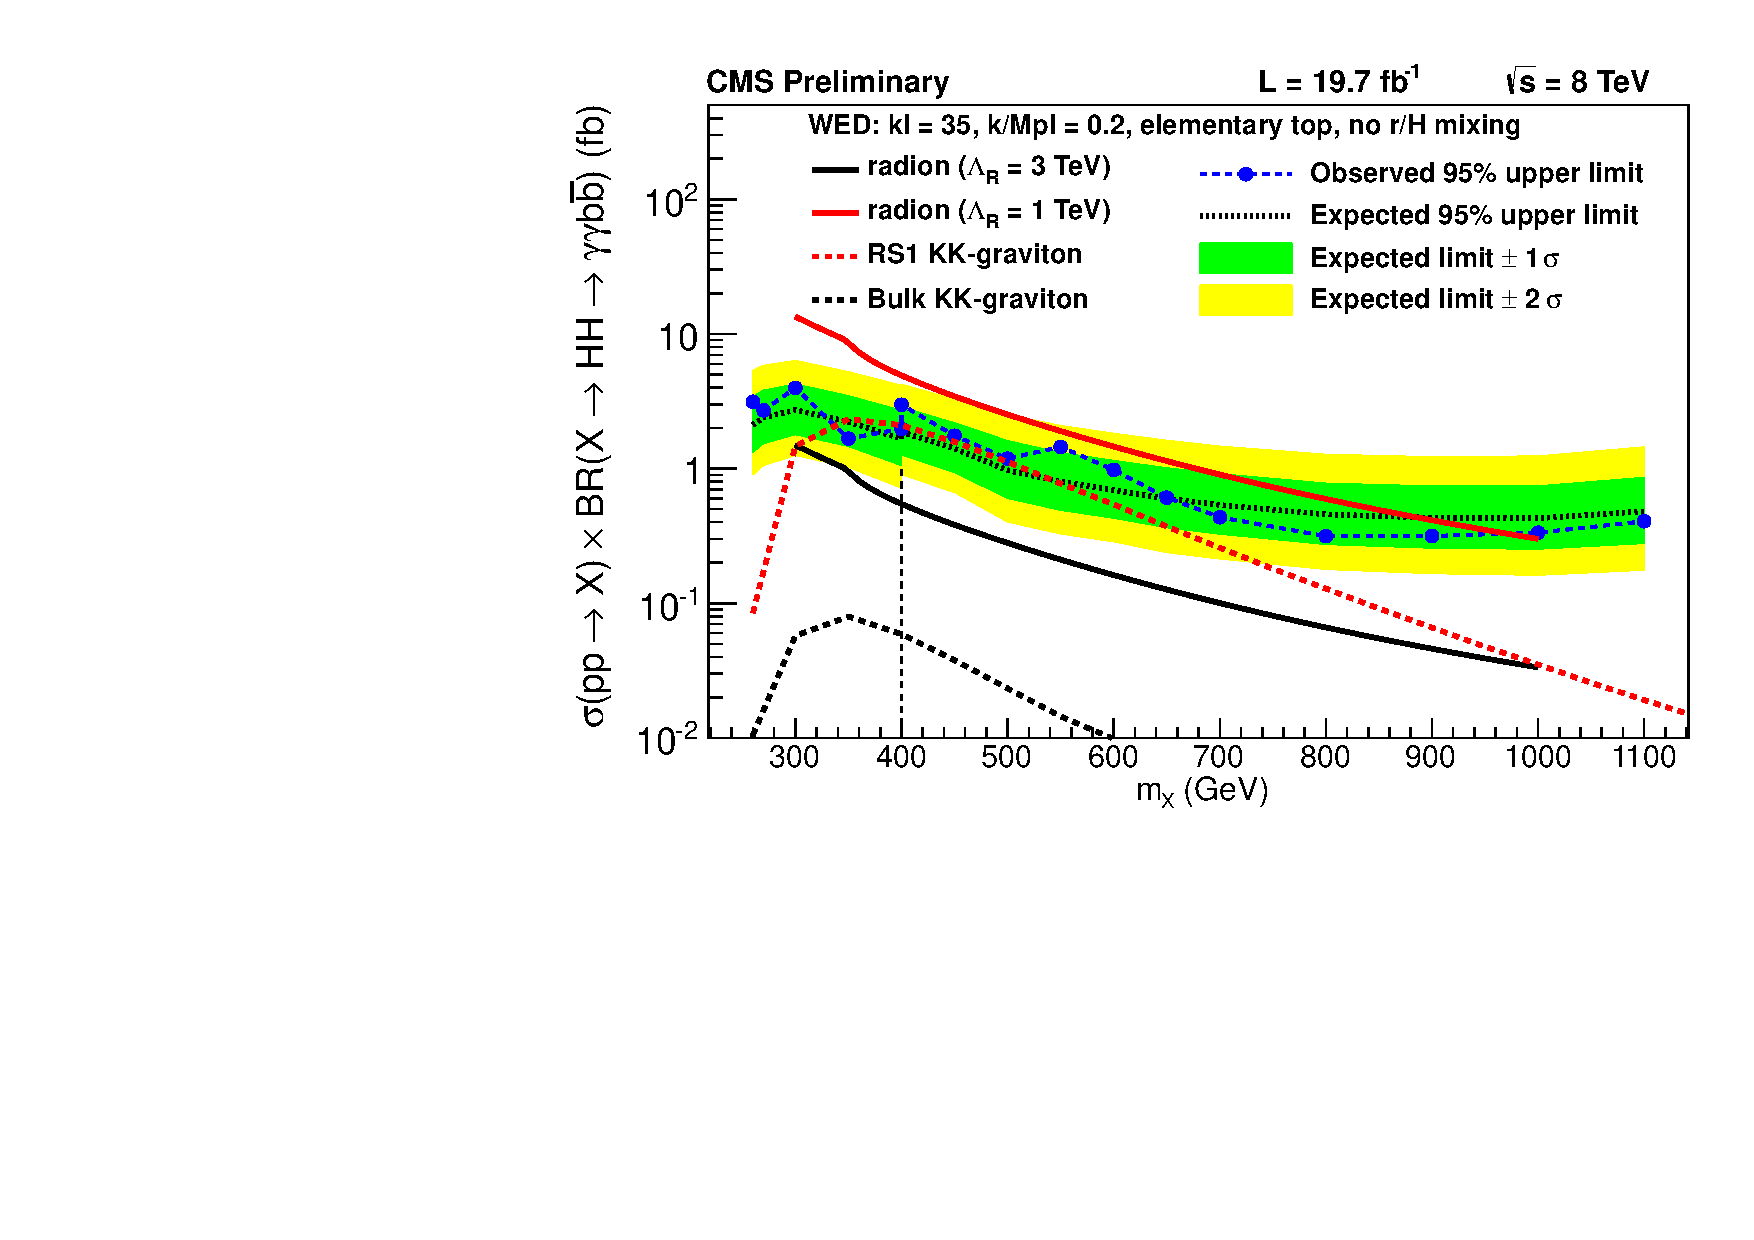
\includegraphics[width=0.8\textwidth]{figures/results/WP4_cutbased_all.pdf}
   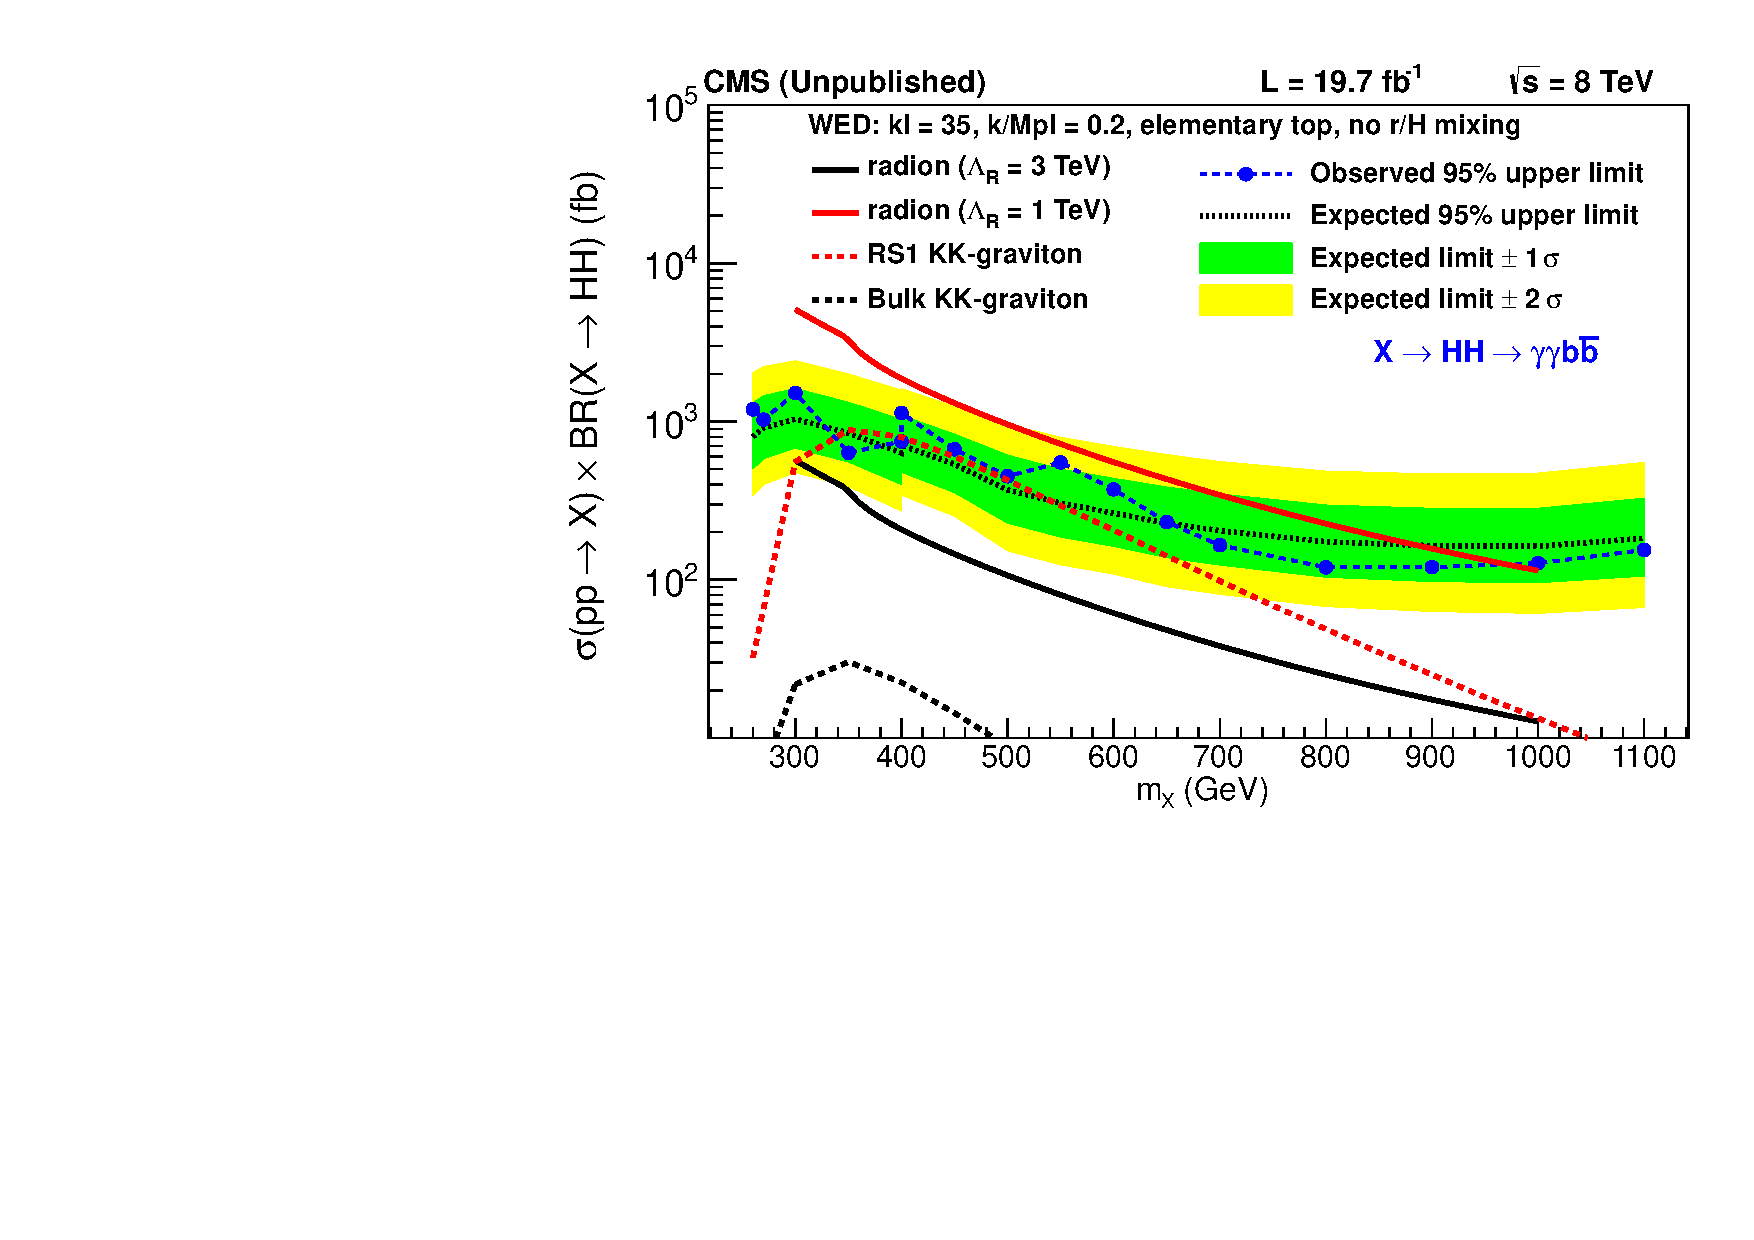
\includegraphics[width=0.8\textwidth]{figures/results/WP4_cutbased_HH.pdf}
 \end{center}
\caption{Expected 95\% CL upper limits on the cross section times branching ratios
$\sigma(pp\rightarrow X) \times \text{BR}( X \rightarrow HH \rightarrow \gamma\gamma b\bar{b})$ (top)
and $\sigma(pp\rightarrow X) \times \text{BR}( X \rightarrow HH )$ (bottom).
Theory lines corresponding to WED models with Radion, RS1 KK-graviton, and bulk KK-graviton are
overlaid. The results are obtained using the asymptotic $\text{CL}_s$ approach.}
\label{fig:limits_allres}
\end{figure}

\subsection{Comparison of Resonant Results}

Figure~\ref{fig:limit_comp} provides a comparison of the observed and expected limits obtained
among several final states in both the CMS and ATLAS Collaborations. The final states compared here
are $\gamma \gamma b\bar{b}$, $b\bar{b}b\bar{b}$, $\tau\tau b\bar{b}$, and multileptons and photons.
The comparison reveals that the $\gamma \gamma b\bar{b}$ is most sensitive to resonant double
Higgs production for $m_X < 400$~GeV, while the $b\bar{b}b\bar{b}$ final state is the most sensitive
for $m_X > 400$~GeV.

\begin{figure}[htbp!]
 \begin{center}
   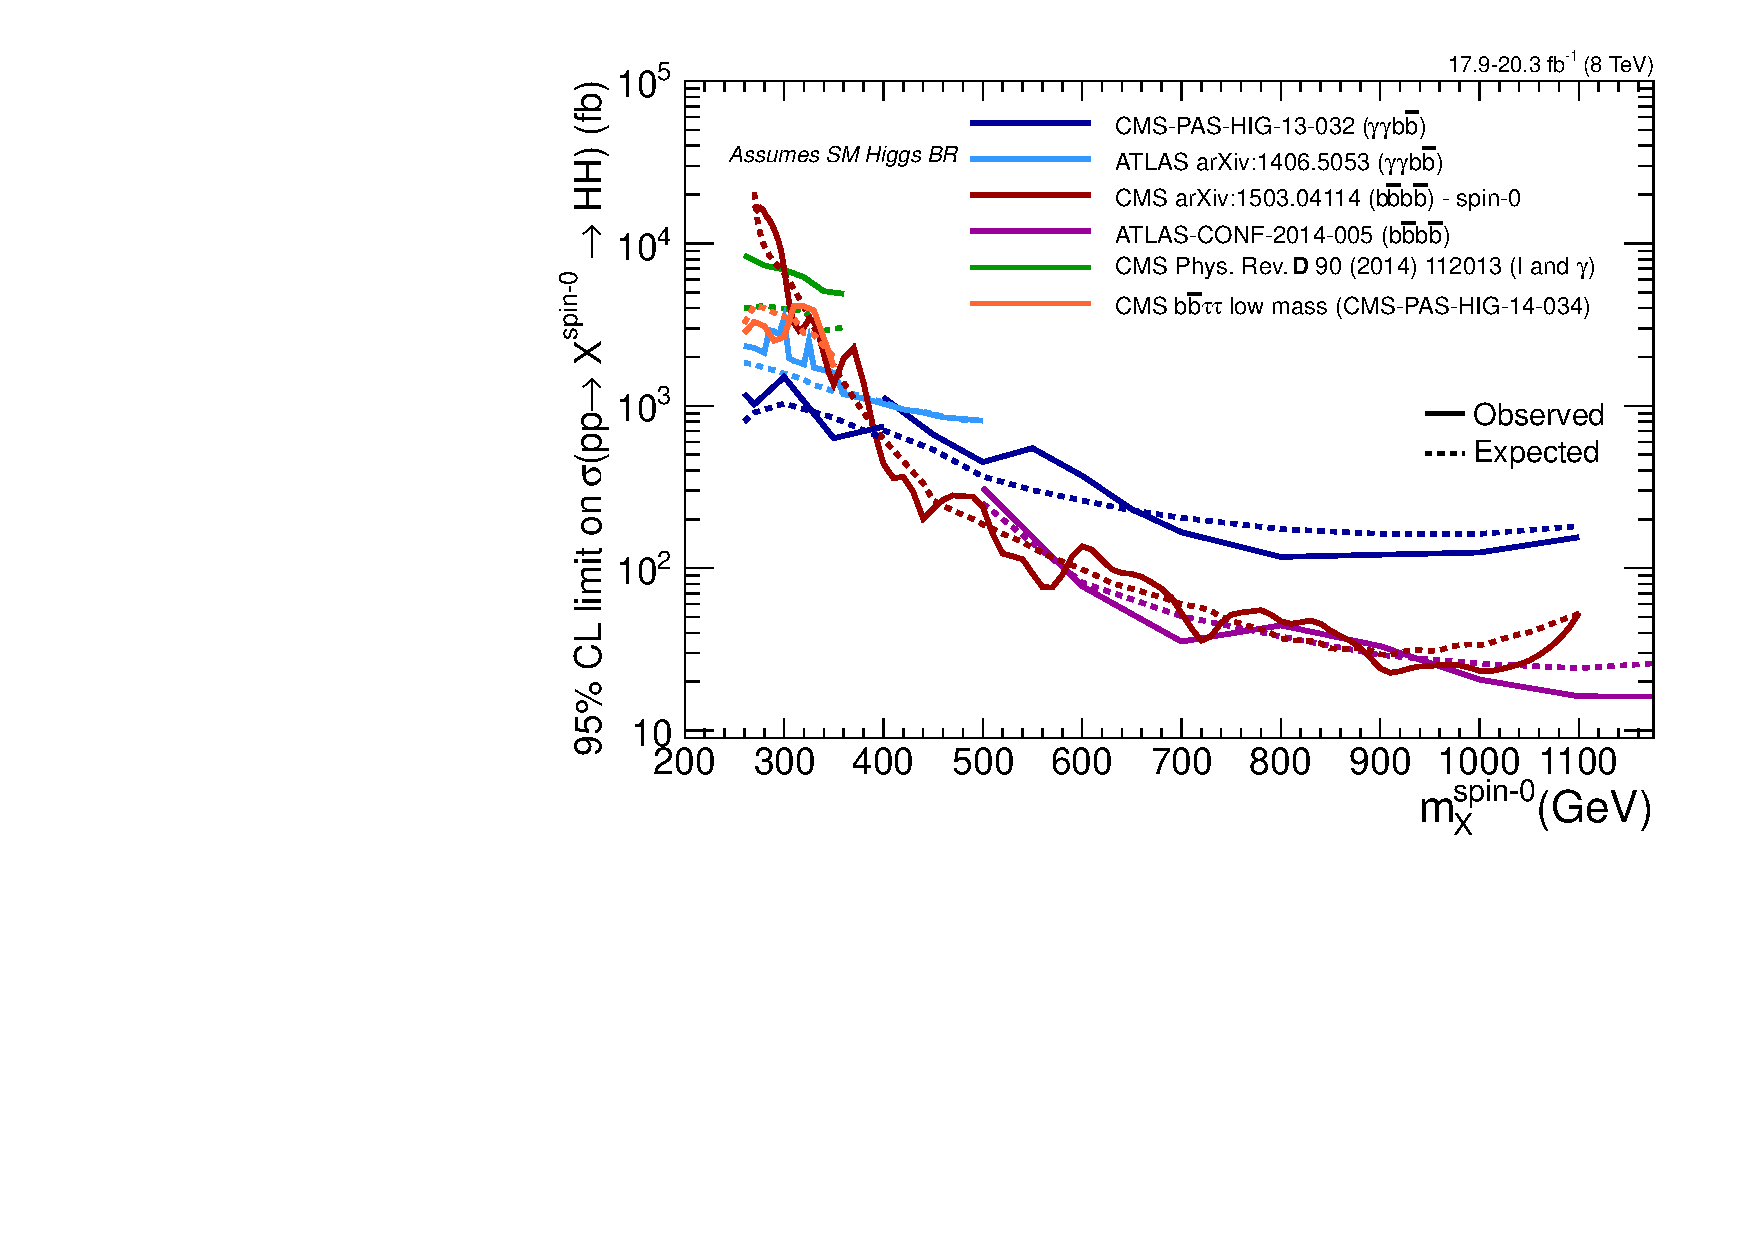
\includegraphics[width=0.9\textwidth]{figures/results/limit_comparison_all.pdf}
 \end{center}
\caption{The observed and expected upper limits of $X_\text{spin-0} \rightarrow HH$ production
at 95\% CL are compared over various searches performed by the CMS and ATLAS Collaborations
looking at the $\gamma \gamma b\bar{b}$~\cite{CMS-PAS-HIG-13-032,Aad:2014yja},
$b\bar{b}b\bar{b}$~\cite{Khachatryan:2015yea,ATLAS-CONF-2014-005},
$\tau\tau b\bar{b}$~\cite{CMS-PAS-HIG-14-034}, and
multileptons and photons~\cite{PhysRevD.90.112013}
final states. As the CMS $b\bar{b}b\bar{b}$ result is dependent on the
resonance spin, the spin-0 result for that analysis is used.}
\label{fig:limit_comp}
\end{figure}

\section{Nonresonant Results\label{sec:nonresresults}}

For the SM nonresonant search,
no excess above the expectation is observed, so an upper limit on the signal cross section is
calculated. The 95\% CL is found using the same approach as in both
regimes of the resonant search. The observed (expected) upper limit on the SM
$pp \rightarrow HH \rightarrow \ggbb$ production cross section is 1.91 fb (1.59 fb).
Assuming SM Higgs branching ratios, the observed (expected) upper limit on SM $pp \rightarrow HH$
production is 726 fb (604 fb). In terms of the SM signal strength modificator $\mu_{HH}$, defined
generally as
\begin{equation}
\mu = \frac{\sigma}{\sigma_\text{SM}} \, ,
\end{equation}
the observed (expected) limit is 72.9 (60.7). These calculations account for the theoretical
uncertainty associated with the SM NNLO cross section.

%\section{The Future\label{sec:future}}

